\begin{figure}[p]
\centering
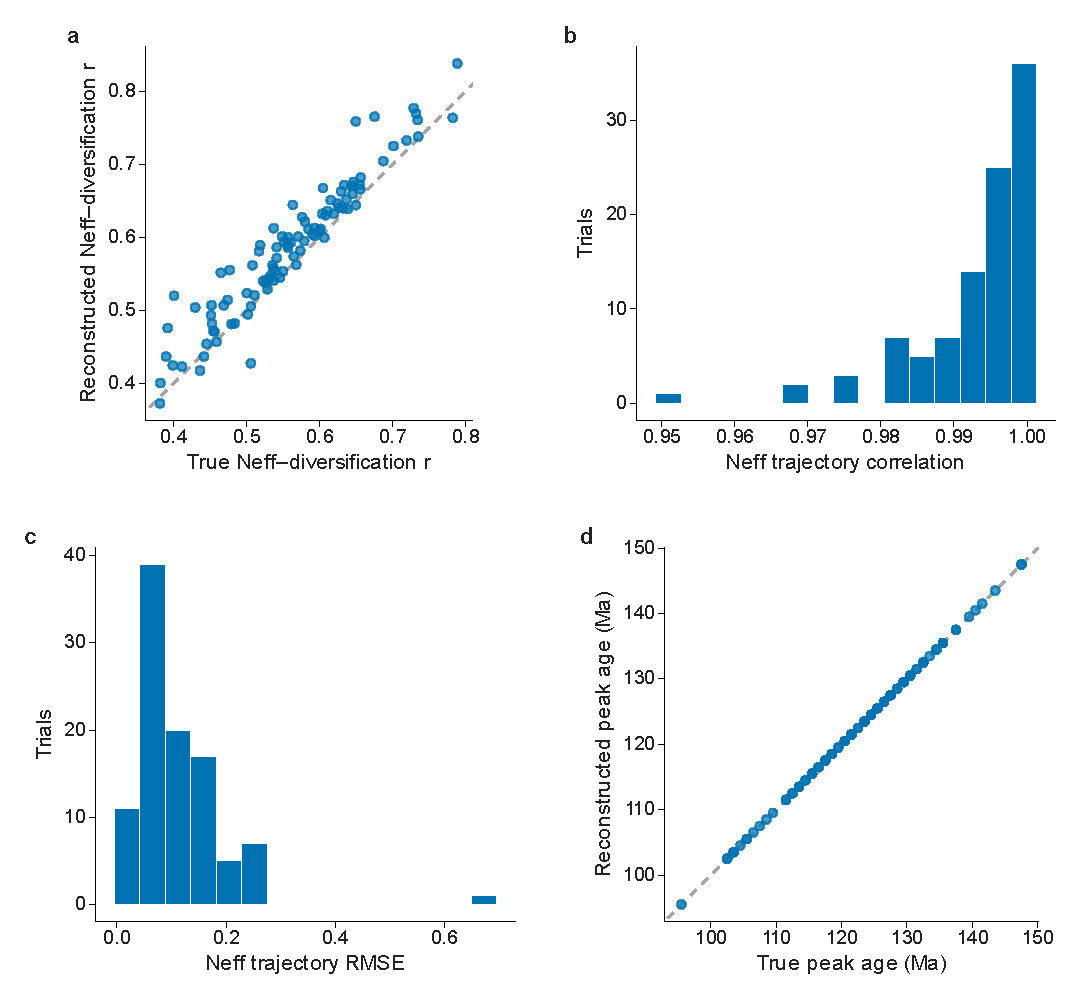
\includegraphics[width=\textwidth]{../figures/recovery-summary.pdf}
\caption{\textbf{Recovery of accelerated phenomic diversity across 100 independent simulations.}
(a) Correlation of true-history and reconstructed $N_{\mathrm{eff}}^{+}$ with
known diversification, each calculated from 15 matched 20-Myr bins.
(b) Correlation between the true and reconstructed diversity trajectories
on the 300-point time grid. (c) Trajectory root-mean-square error.
(d) True and reconstructed peak ages; where maxima are tied, the oldest
maximizing grid point is reported. Dashed lines in (a,d) indicate equality.
Each point or histogram observation represents one trial. Truth includes
all 200 simulated characters; reconstruction uses characters remaining
variable at the tips.}
\label{fig:neff-recovery}
\end{figure}

\begin{figure}[p]
\centering
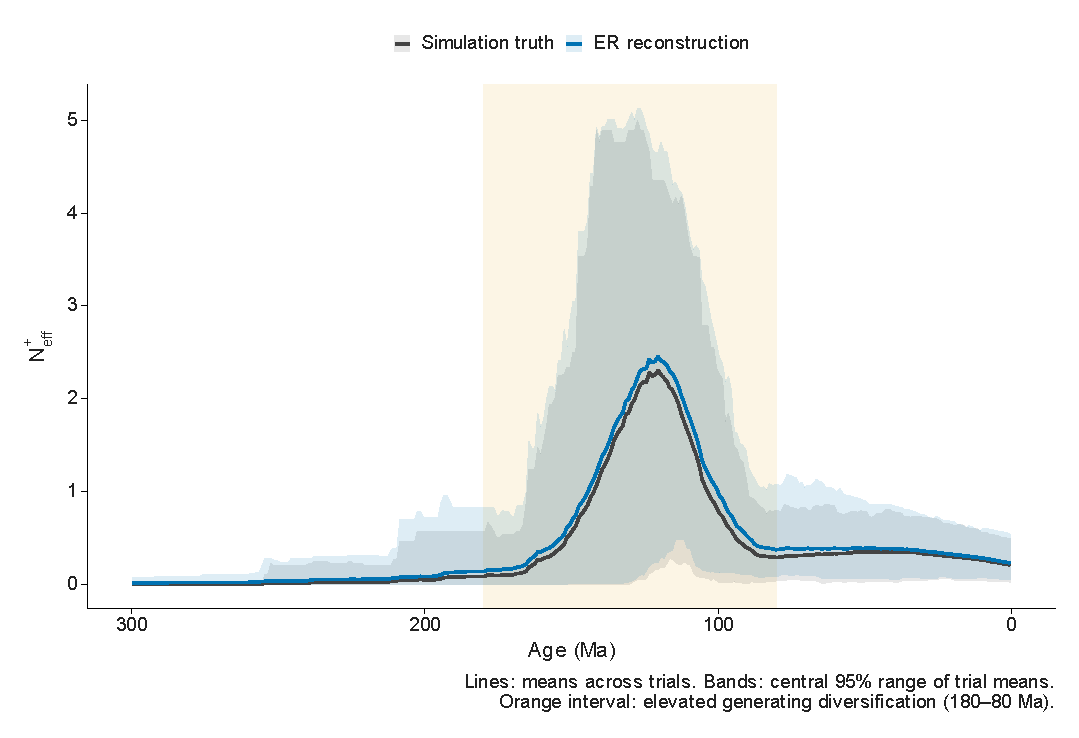
\includegraphics[width=\textwidth]{../figures/neff-through-time.pdf}
\caption{\textbf{True and reconstructed diversity through time.}
Lines show means across the 100 trial trajectories, and bands show their
pointwise central 95\% range. These bands quantify among-trial variation,
not uncertainty in the grand mean. Orange shading marks the 180--80~Ma
interval of elevated generating speciation. Diversity can peak within a
narrower interval because the ten focal branches overlap over only part of
the elevated-rate epoch. True-history metrics use realized changes averaged
over whole branches, rather than exact event-time densities.}
\label{fig:neff-curves}
\end{figure}

\begin{figure}[p]
\centering
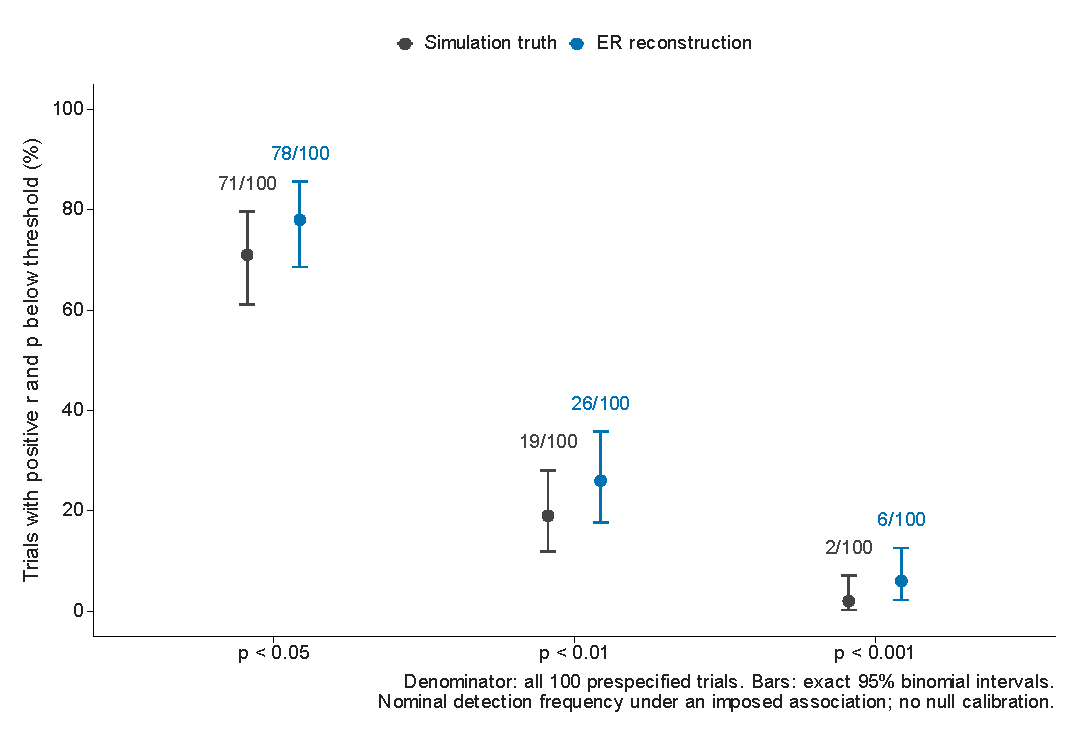
\includegraphics[width=\textwidth]{../figures/p-value-percentages.pdf}
\caption{\textbf{Nominal detection frequency under the imposed association.}
Points show the percentage of all 100 trials with a positive Pearson
correlation and a two-sided $p$-value below each threshold; labels give
counts over the full denominator. Bars are exact 95\% binomial intervals.
Grey denotes true-history diversity and blue reconstructed diversity.
Individual tests use 15 matched 20-Myr bins and are not corrected for
temporal autocorrelation. These frequencies therefore do not establish
false-positive-calibrated power. The complete tables also report
significance irrespective of correlation sign, unavailable tests, and
percentages among estimable tests.}
\label{fig:neff-detection}
\end{figure}

\begin{figure}[p]
\centering
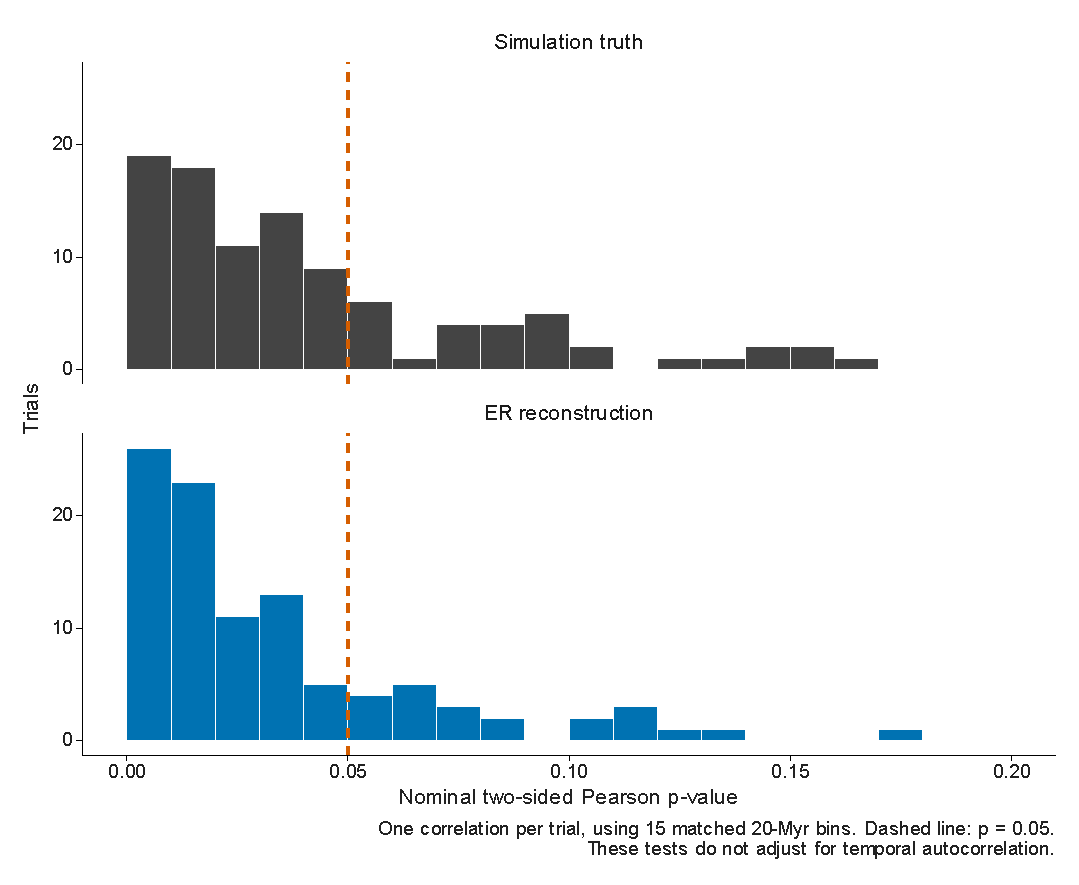
\includegraphics[width=\textwidth]{../figures/p-value-distribution.pdf}
\caption{\textbf{Distribution of nominal Pearson $p$-values.}
Each panel contains the trial-wise two-sided $p$-values for the strict
acceleration definition. The dashed line marks $p=0.05$. Tests compare
true-history or reconstructed diversity against the same known generating
diversification trajectory; no diversification parameter was estimated.}
\label{fig:neff-pvalues}
\end{figure}

\begin{figure}[p]
\centering
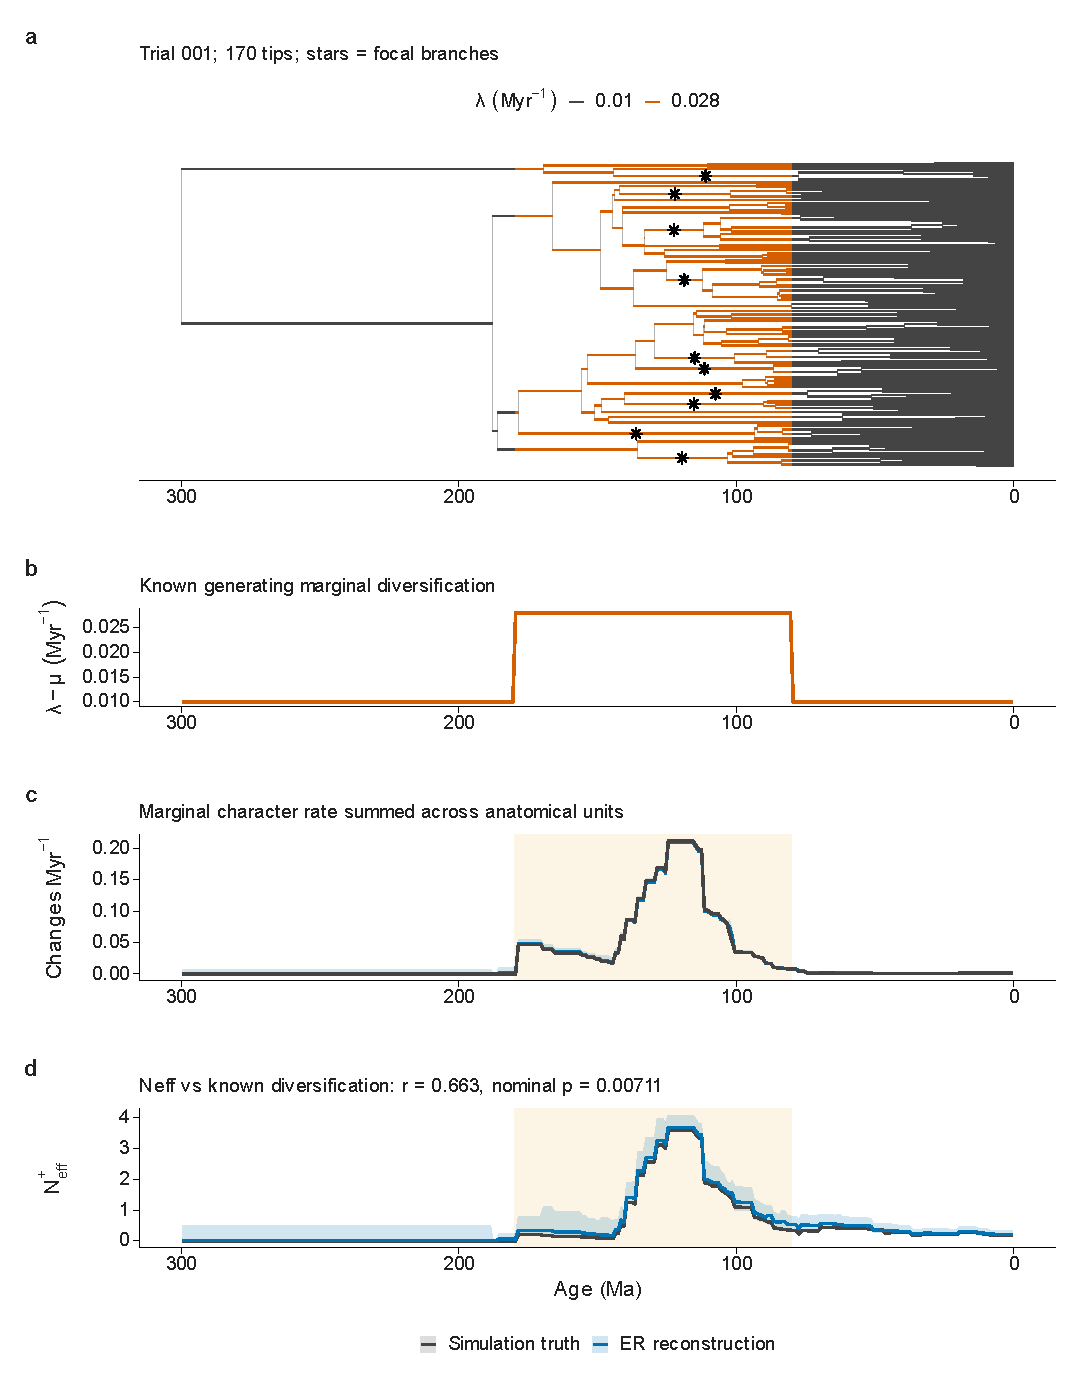
\includegraphics[width=.88\textwidth]{../figures/trial-001-overview.pdf}
\caption{\textbf{Simulation and reconstruction for prespecified trial~001.}
(a) Simulated tree, with each branch segment coloured by its generating
speciation rate; stars mark the ten focal branches. (b) Known marginal
net diversification. (c) Marginal character-change rate summed across the
ten units. (d) Accelerated phenomic diversity, with the reconstructed
Neff--diversification correlation and nominal $p$-value. Grey curves use
actual simulated histories; blue curves use reconstructed histories.
Within-trial bands are central 95\% conditional mapping intervals.
The tree, diversification trajectory and true histories are simulated;
character rates and diversity shown in blue are inferred from tip states.
This trial was chosen by ID before inspecting its results.}
\label{fig:neff-example}
\end{figure}

\begin{figure}[p]
\centering
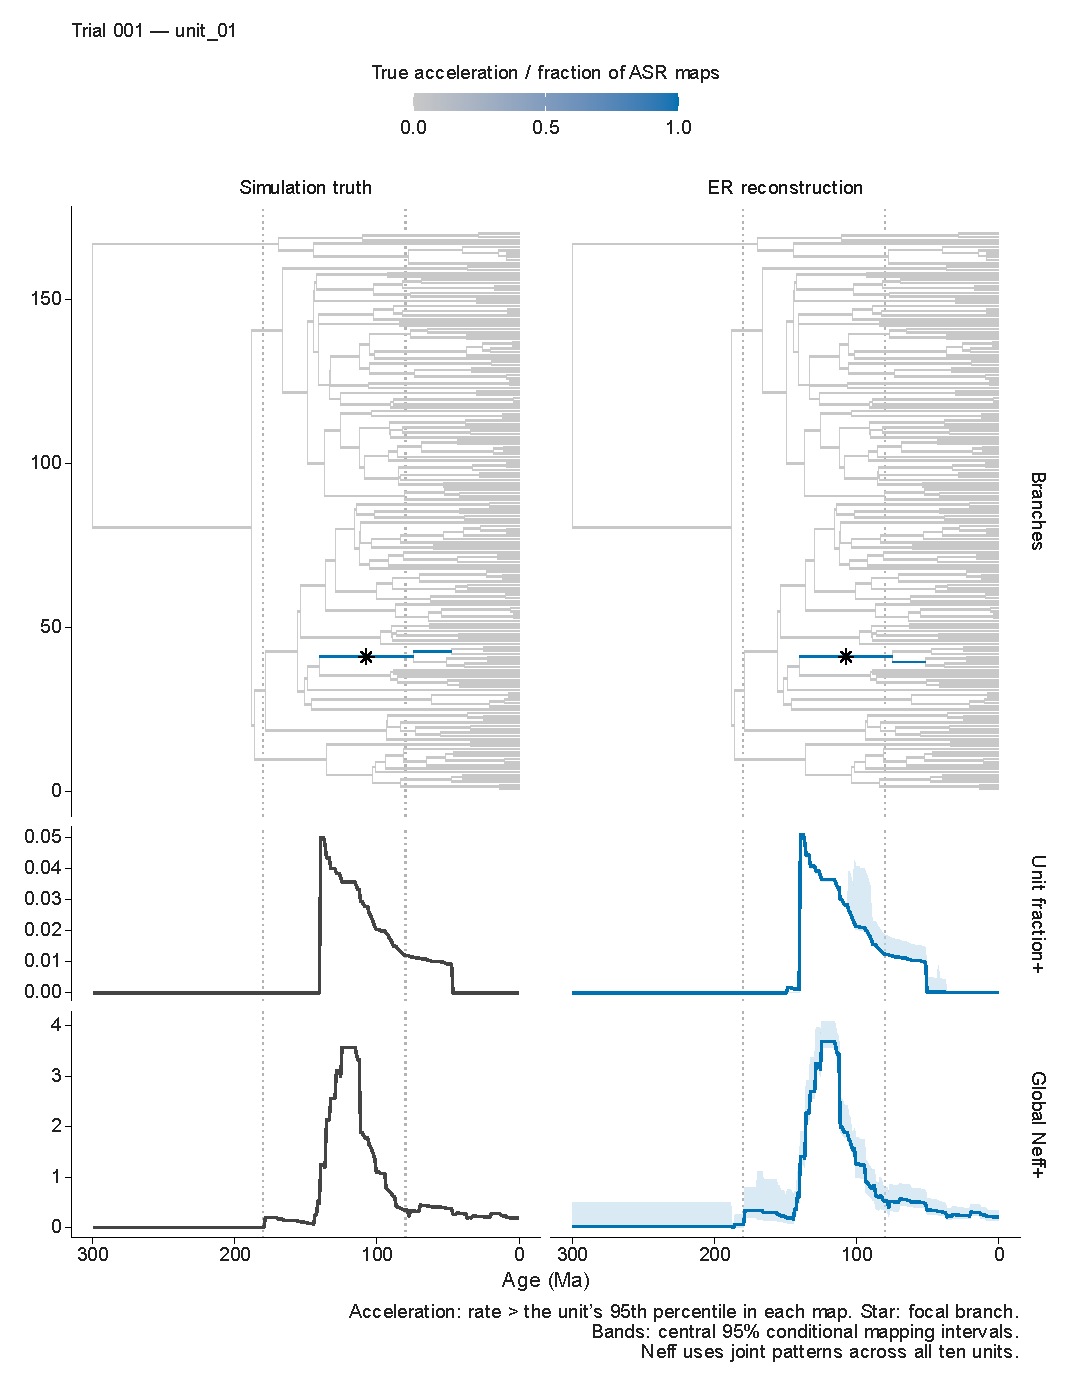
\includegraphics[page=1,width=.88\textwidth]{../figures/trial-001-unit-acceleration.pdf}
\caption{\textbf{Unit-level acceleration and its alignment with global diversity.}
The first page of the ten-unit atlas for trial~001 is shown.
Left: true-history acceleration indicators; right: the fraction of
conditional maps classifying each branch as accelerated. The star marks
the focal branch. Middle panels show the fraction of contemporaneous
branches accelerated for this unit; lower panels show global
$N_{\mathrm{eff}}^{+}$ computed from joint patterns across all ten units.
Bands describe conditional mapping variation; colours on reconstructed
branches are classification frequencies, not significance tests.
Dotted guides bound the elevated diversification epoch. The complete
atlas contains one page per unit; companion PDFs show trajectories and
full diagnostics for every trial.}
\label{fig:neff-unit}
\end{figure}
